\chapter{\LaTeX \, Reference}
\section{Xcolor}

\begin{note}[{Color Note 1}]\\
How does a mixture of $40\%$ green and $60\%$ yellow look like?\\
(Answer: $40\%$ \tikz \draw[fill=green] (0,0) rectangle (6mm,3mm);
$+ 60\%$ \tikz \draw[fill=yellow] (0,0) rectangle (6mm,3mm);
$=$ \tikz \draw[fill=green!40!yellow] (0,0) rectangle (6mm,3mm);
e.g., \verb|\color{green!40!yellow} |)
\end{note}
\begin{note}[{Color Note 2}]\\
And how does its complementary color look like?\\
 (Answer:  \tikz \draw[fill=-green!40!yellow] (0,0) rectangle (6mm,3mm);
accessible via \verb|\color{-green!40!yellow} |)
\end{note}
\begin{note}[{Color Note 3}]\\
Now mix three parts of last color with two parts of its complement and one part of red, PLZ!:\\
(Answer: $3 \times $ \tikz \draw[fill=-green!40!yellow] (0,0) rectangle (6mm,3mm);
$+ 2 \times$ \tikz \draw[fill=green!40!yellow] (0,0) rectangle (6mm,3mm);
$+ 1 \times$ \tikz \draw[fill=red] (0,0) rectangle (6mm,3mm);
$=$ \tikz \draw[fill={rgb:-green!40!yellow,3;green!40!yellow,2;red,1}] (0,0) rectangle (6mm,3mm);
\\ e.g., \verb|\color{rgb:-green!40!yellow,3;green!40!yellow,2;red,1} |)
\end{note}
\section{Tikz}

\begin{note}[Tiks inline commands]: 
use \textbf{\textbackslash tikz} for simple inline commands
\end{note}
	
\begin{note}[Draw]: \\
use \textbf{\textbackslash draw} to draw a line\\
\verb|\tikz \draw (0pt,0pt) -- (20pt,6pt);|
\tikz \draw (0pt,0pt) -- (20pt,6pt);
\\
\verb|\tikz \draw (0pt,0pt) -- (20pt,0pt);|
\tikz \draw (0pt,0pt) -- (20pt,0pt);
\\
\verb|\tikz \draw (0pt,0pt) -- (0pt,20pt);|
\tikz \draw (0pt,0pt) -- (0pt,20pt);
\end{note}

\begin{note}[\textbackslash fill and \textbackslash circle usage]:\\
	\verb|\tikz \fill[orange] (0,0) circle (1ex);|
	\tikz \fill[orange] (0,0) circle (1ex); 
\end{note}
\begin{note}[Large pictures]:\\
use \textbf{\textbackslash begin\{tikzpivture\}} and \textbf{\textbackslash end\{tikzpicture\}} for larger pictures
\begin{table}[h]
\centering
\begin{tabular}{c|c}
\begin{lstlisting}[language={[LaTeX]TeX},basicstyle=\ttfamily]
\draw[style=dashed] (2,.5) circle (0.5);
\draw[fill=green!50] (1,1)
ellipse (.5 and 1);
\draw[fill=blue] (0,0) rectangle (1,1);
\draw[style=thick]
(3,.5) -- +(30:1) arc(30:80:1) -- cycle;
\end{lstlisting} &
	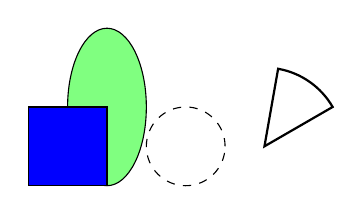
\begin{tikzpicture}
	\draw[style=dashed] (2,.5) circle (0.5);
	\draw[fill=green!50] (1,1)
	ellipse (.5 and 1);
	\draw[fill=blue] (0,0) rectangle (1,1);
	\draw[style=thick]
	(3,.5) -- +(30:1) arc(30:80:1) -- cycle;
	\end{tikzpicture}
\end{tabular}
\end{table}
\end{note}
	
\begin{note}[Cordinate System]:
\begin{itemize}
\item It Starts from lower left
\item To make boundaries visible use :
\begin{lstlisting}
\hspace*{..}, \vspace*{..}
\end{lstlisting}
\item sample:
\begin{lstlisting}
\vspace{-1cm}\hspace{8cm}
\begin{tikzpicture}[ scale=.8, show background rectangle]
\draw (2,2) circle (1);
\draw (0 mm, 0 pt) -- (16 em, 1);
\end{lstlisting}
\vspace{-1cm}\hspace{8cm}
\begin{tikzpicture}[ scale=.8, show background rectangle]
\draw (2,2) circle (1);
\draw (0 mm, 0 pt) -- (16 em, 1);
\end{tikzpicture}
\end{itemize}
\begin{remark}
A solution in the spirit of \LaTeX \, would be the use of a multicolumn environment or of minipages. But sometimes the 
\textbf{\textbackslash hspace \textbackslash vspace} hack is faster and more flexible.)
\end{remark}
\end{note}
	
\begin{note}[Paths]:\\

\begin{tabular}{c l}
\tikz \path[draw] (1,1) -- (2,2) -- (3,1); &
\begin{lstlisting}
\tikz \path[draw] (1,1) -- (2,2) -- (3,1);
\end{lstlisting} \\
\tikz \path[draw,line width=4pt] (1,1) -- (2,2)--(3,1)--cycle; &
\begin{lstlisting}
\tikz \path[draw,line width=4pt] (1,1) -- (2,2)--(3,1)--cycle;
\end{lstlisting} \\
\tikz \path[draw, fill=green!20] (1,1) -- (2,2) -- (3,1) --cycle; &
\begin{lstlisting}
\tikz \path[draw, fill=green!20] (1,1) -- (2,2) -- (3,1) --cycle;
\end{lstlisting} \\
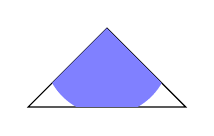
\begin{tikzpicture}
\path[clip, draw] (1,1)--(2,2)--(3,1)--cycle;
\path[fill=blue!50] (2, 1.7) circle (.8);
\end{tikzpicture} &
\begin{lstlisting}
\path[clip, draw] (1,1)--(2,2)--(3,1)--cycle;
\path[fill=blue!50] (2, 1.7) circle (.8);
\end{lstlisting}
\end{tabular}
\end{note}
	
\begin{note}[Shading]:\\
	
	\begin{tabular}{c l}
		\tikz \path[shade,draw] (1,1) -- (2,2)--(3,1)--cycle; &
\begin{lstlisting}
\tikz \path[shade,draw] (1,1) -- (2,2)--(3,1)--cycle;
\end{lstlisting} \\
		\tikz \shade[left color=red] (1,1)--(2,2)--(3,1)--cycle; &
\begin{lstlisting}
\tikz \shade[left color=red] (1,1)--(2,2)--(3,1)--cycle;
\end{lstlisting} \\
		\tikz \shade[top color=red, bottom color=green]
		(0,0) rectangle (2,1); &
\begin{lstlisting}
\tikz \shade[top color=red, bottom color=green]
(0,0) rectangle (2,1);
\end{lstlisting} \\
		\tikz \shade[draw,shading=radial, inner color=blue]
		(0,0) rectangle (2,1); &
\begin{lstlisting}
\tikz \shade[draw,shading=radial, inner color=blue]
(0,0) rectangle (2,1);;
\end{lstlisting} \\
		\tikz \shade[shading=ball, ball color=blue]
		(0,0) rectangle (2,1); &
\begin{lstlisting}
\tikz \shade[shading=ball, ball color=blue]
(0,0) rectangle (2,1);
\end{lstlisting} \\
		
\begin{tikzpicture}
		\shade[shading=ball, ball color=blue] (0,0) circle (.3);
		\shade[shading=ball, ball color=white] (1,0) circle (.3);
		\shade[shading=ball, ball color=black] (2,0) circle (.3);
		\end{tikzpicture} &
\begin{lstlisting}
\shade[shading=ball, ball color=blue] (0,0) circle (.3);
\shade[shading=ball, ball color=white] (1,0) circle (.3);
\shade[shading=ball, ball color=black] (2,0) circle (.3);
\end{lstlisting}
	\end{tabular}
\end{note}
\begin{note}[Polar Coordinates]:\\

\begin{tabular}{c | l}
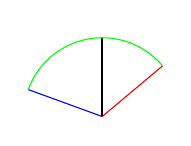
\begin{tikzpicture}
\draw[color=red] (0,0) -- (40:1);
\draw[color=blue] (0,0) -- (160:1);
\draw[thick] (0,0) -- (90:1);
\draw[color=green] (40:1) arc (40:160:1);
\end{tikzpicture} &
\begin{lstlisting}
\draw[color=red] (0,0) -- (40:1);
\draw[color=blue] (0,0) -- (160:1);
\draw[thick] (0,0) -- (90:1);
\draw[color=green] (40:1) arc (40:160:1);
\end{lstlisting}
\end{tabular}
\end{note}
\begin{note}[Curved Lines]:\\

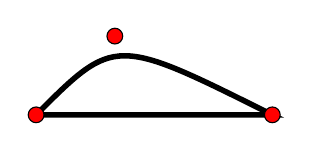
\begin{tikzpicture}
\draw[line width=2pt] (0, 0) .. controls(1,1) .. (3, 0) --cycle;
\draw[fill = red] (0,0) circle (1mm);
\draw[fill = red] (1,1) circle (1mm);
\draw[fill = red] (3,0) circle (1mm);
\end{tikzpicture}
\begin{lstlisting}
\draw[line width=2pt] (0, 0) .. controls(1,1) .. (3, 0) --cycle;
\end{lstlisting} 


\begin{tikzpicture}
\draw[line width=8pt] (0, 0) ..
controls(1, 0) and (1, 1)
.. (0, 1);
\draw[fill = red] (0,0) circle (1mm);
\draw[fill = red] (1,0) circle (1mm);
\draw[fill = red] (1,1) circle (1mm);
\draw[fill = red] (0,1) circle (1mm);
\end{tikzpicture}
\begin{lstlisting}
\draw[line width=8pt] (0, 0) ..
		controls(1, 0) and (1, 1)
			.. (0, 1);
\end{lstlisting} 

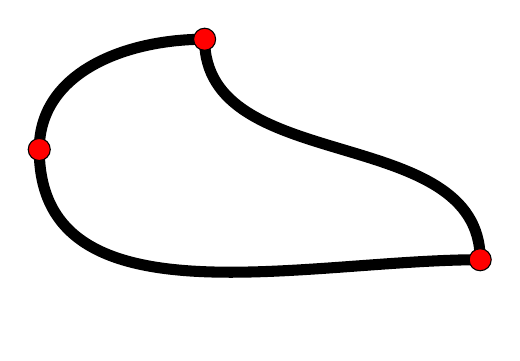
\begin{tikzpicture}[scale=.7]
\draw[line width=4pt] (0,0) to [out=90, in=180] (3,2)
							to [out=-90, in=90] (8,-2)
							to [out=180, in=-90] (0,0);
\draw[fill = red] (0,0) circle (2mm);
\draw[fill = red] (3,2) circle (2mm);
\draw[fill = red] (8,-2) circle (2mm);
\end{tikzpicture}
\begin{lstlisting} [language={[LaTeX]TeX},basicstyle=\ttfamily]
\draw[line width=4pt] (0,0) to [out=90, in=180] (3,2)
				to [out=-90, in=90] (8,-2)
				to [out=180, in=-90] (0,0);
\end{lstlisting} 
\end{note}
\begin{note}[Arrows, Dash patterns]:\\
\begin{tabular}{c l}
\tikz \draw[->] (0,0) -- (1,0); &
\begin{lstlisting} [language={[LaTeX]TeX},basicstyle=\ttfamily]
\tikz \draw[->] (0,0) -- (1,0);
\end{lstlisting} \\

\tikz \draw[dotted, >->>] (0,0) -- (1,0); &
\begin{lstlisting} [language={[LaTeX]TeX},basicstyle=\ttfamily]
\tikz \draw[dotted, >->>] (0,0) -- (1,0);
\end{lstlisting} \\

\tikz \draw[|<->|] (0,0) -- (1,0); &
\begin{lstlisting} [language={[LaTeX]TeX},basicstyle=\ttfamily]
\tikz \draw[|<->|] (0,0) -- (1,0);
\end{lstlisting} \\

\tikz \draw[dashed, o-)] (0,0) -- (1,0); &
\begin{lstlisting} [language={[LaTeX]TeX},basicstyle=\ttfamily]
\tikz \draw[dashed, o-)] (0,0) -- (1,0);
\end{lstlisting} \\

\tikz \draw[loosely dashed] (0,0) -- (1,0); &
\begin{lstlisting} [language={[LaTeX]TeX},basicstyle=\ttfamily]
\tikz \draw[loosely dashed] (0,0) -- (1,0);
\end{lstlisting} \\

\tikz \draw[densely dotted] (0,0) -- (1,0); &
\begin{lstlisting} [language={[LaTeX]TeX},basicstyle=\ttfamily]
\tikz \draw[densely dotted] (0,0) -- (1,0);
\end{lstlisting} \\

\tikz \draw[->] (0,0) .. controls (.2,-.2) .. (1, 0); &
\begin{lstlisting} [language={[LaTeX]TeX},basicstyle=\ttfamily]
\tikz \draw[->] (0,0) .. controls (.2,-.2) .. (1, 0);
\end{lstlisting} \\
\end{tabular}
\end{note}
	
\begin{note}[Clipping and Scope]\\

\begin{itemize}
\item After a \textbf{\textbackslash Clip} Command,all subsequent drawings are clipped, only the parts
inside the clipping region are drawn.
\item Use the \textbf{Scope} environment to restrict the effect of clipping
\end{itemize}

\begin{tabular}{c|l}
	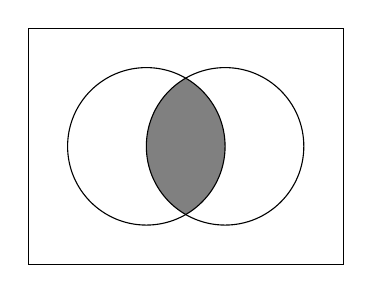
\begin{tikzpicture}
	\draw (-2, 1.5) rectangle (2, -1.5);
	\begin{scope}
	\clip (-0.5, 0) circle (1);
	\clip ( 0.5, 0) circle (1);
	\fill[color=gray] (-2,1.5)
	rectangle (2,-1.5);
	\end{scope}
	\draw (-0.5, 0) circle (1);
	\draw ( 0.5, 0) circle (1);
	\end{tikzpicture} &
\begin{lstlisting} [language={[LaTeX]TeX},basicstyle=\ttfamily]
\draw (-2, 1.5) rectangle (2, -1.5);
\begin{scope}
\clip (-0.5, 0) circle (1);
\clip ( 0.5, 0) circle (1);
\fill[color=gray] (-2,1.5) rectangle (2,-1.5);
\end{scope}
\draw (-0.5, 0) circle (1);
\draw ( 0.5, 0) circle (1);
\end{lstlisting} \\
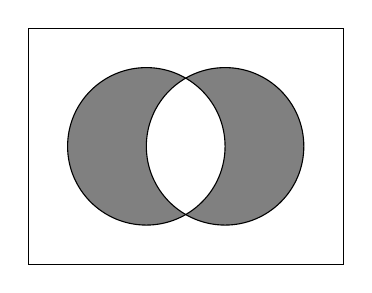
\begin{tikzpicture}
\draw (-2, 1.5) rectangle (2, -1.5);
\fill[color=gray] (-0.5, 0) circle (1);
\fill[color=gray] ( 0.5, 0) circle (1);
\begin{scope}
\clip (-0.5, 0) circle (1);
\clip ( 0.5, 0) circle (1) ;
\draw[fill=white] (-2,1.5)
rectangle (2,-1.5);
\end{scope}
\draw (-0.5, 0) circle (1);
\draw ( 0.5, 0) circle (1);
\end{tikzpicture} &
\begin{lstlisting} [language={[LaTeX]TeX},basicstyle=\ttfamily]
\draw (-2, 1.5) rectangle (2, -1.5);
\fill[color=gray] (-0.5, 0) circle (1);
\fill[color=gray] ( 0.5, 0) circle (1);
\begin{scope}
\clip (-0.5, 0) circle (1);
\clip ( 0.5, 0) circle (1) ;
\draw[fill=white] (-2,1.5) rectangle (2,-1.5);
\end{scope}
\draw (-0.5, 0) circle (1);
\draw ( 0.5, 0) circle (1);
\end{lstlisting} 
\end{tabular}
\end{note}
	
\begin{note}[Nodes]:
\begin{itemize}
\item Nodes are added to paths after the path is drawn:
\tikz \path[draw] (0, 0) node {A} -- (1,0) -- (1,1) node {B};
\begin{lstlisting}[language={[LaTeX]TeX},basicstyle=\ttfamily]
\tikz \path[draw] (0, 0) node {A} -- (1,0) -- (1,1) node {B};
\end{lstlisting}	
\item Nodes can get a name for later references. Nodes have many options.
\begin{tikzpicture}
\path[draw] (0, 0) node[draw] (nodeA) {$A^2$} -- (1,0)
-- (1,1) node[ellipse,fill=green](nodeB) {\tiny B};
\draw[red,->] (nodeA) -- (nodeB);
\end{tikzpicture}
\begin{lstlisting}[language={[LaTeX]TeX},basicstyle=\ttfamily]
\path[draw] (0, 0) node[draw] (nodeA) {$A^2$} -- (1,0)
-- (1,1) node[ellipse,fill=green](nodeB) {\tiny B};
\draw[red,->] (nodeA) -- (nodeB);
\end{lstlisting}

\item Another Sample \\

\begin{tabular}{c l}
\begin{tikzpicture}
\begin{tikzpicture}[scale=.9, transform shape]
\tikzstyle{every node} = [circle, fill=gray!30]
\node (a) at (0, 0) {A};
\node (b) at +(0: 1.5) {B};
\node (c) at +(60: 1.5) {C};
\foreach \from/\to in {a/b, b/c, c/a}
\draw [->] (\from) -- (\to);
\end{tikzpicture}
\end{tikzpicture} &
\begin{lstlisting} [language={[LaTeX]TeX},basicstyle=\ttfamily]
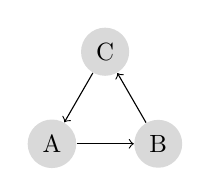
\begin{tikzpicture}[scale=.9, transform shape]
\tikzstyle{every node} = [circle, fill=gray!30]
\node (a) at (0, 0) {A};
\node (b) at +(0: 1.5) {B};
\node (c) at +(60: 1.5) {C};
\foreach \from/\to in {a/b, b/c, c/a}
	\draw [->] (\from) -- (\to);
\end{tikzpicture}
\end{lstlisting} 	
\end{tabular}
\item Nodes on a path can have a placement option\\

\begin{tabular}{c | l}

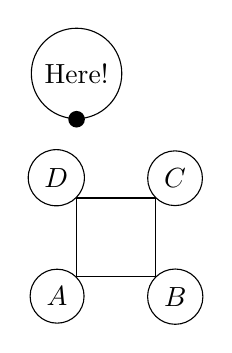
\begin{tikzpicture}
\fill (0,2) circle (3pt) node[above] {Here!};
\draw (0,0) node[below left] {$A$} --
(1,0) node[below right] {$B$} --
(1,1) node[above right] {$C$} --
(0,1) node[above left] {$D$} -- cycle;
\end{tikzpicture} &
\begin{lstlisting} [language={[LaTeX]TeX},basicstyle=\ttfamily]
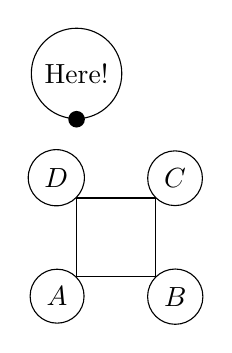
\begin{tikzpicture}
\fill (0,2) circle (3pt) node[above] {Here!};
\draw (0,0) node[below left] {$A$} --
(1,0) node[below right] {$B$} --
(1,1) node[above right] {$C$} --
(0,1) node[above left] {$D$} -- cycle;
\end{tikzpicture}
\end{lstlisting}\\
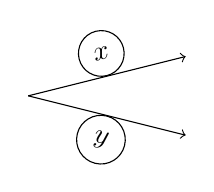
\begin{tikzpicture}
\draw[->] (0,0) -- (2,0.5) node[pos=.5,sloped,above] {$x$};
\draw[->] (0,0) -- (2,-.5) node[pos=.5,sloped,below] {$y$};
\end{tikzpicture} &
\begin{lstlisting} [language={[LaTeX]TeX},basicstyle=\ttfamily]
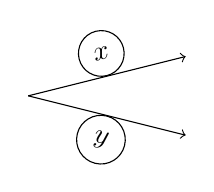
\begin{tikzpicture}
\draw[->] (0,0) -- (2,0.5) node[pos=.5,sloped,above] {$x$};
\draw[->] (0,0) -- (2,-.5) node[pos=.5,sloped,below] {$y$};
\end{tikzpicture}
\end{lstlisting}\\
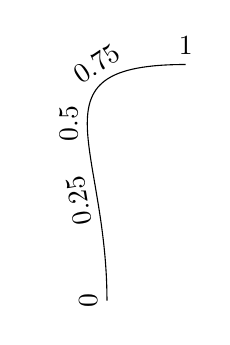
\begin{tikzpicture}
\tikzstyle{every node} = [sloped,above, %
allow upside down]
\draw (0,0).. controls +(up:2cm) and +(left:2cm) ..(1,3)
\foreach \p in {0,0.25,...,1} {node[pos=\p]{\p}};
\end{tikzpicture} &
\begin{lstlisting} [language={[LaTeX]TeX},basicstyle=\ttfamily]
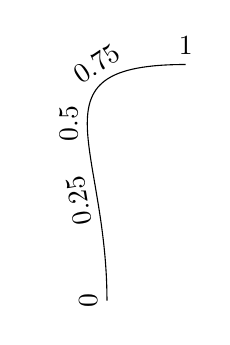
\begin{tikzpicture}
\tikzstyle{every node} = [sloped,above, %
allow upside down]
\draw (0,0).. controls +(up:2cm) and +(left:2cm) ..(1,3)
\foreach \p in {0,0.25,...,1} {node[pos=\p]{\p}};
\end{tikzpicture}
\end{lstlisting}
\end{tabular}
\item Simple computations are possible inside TikZ \\

\begin{tabular}{c|l}

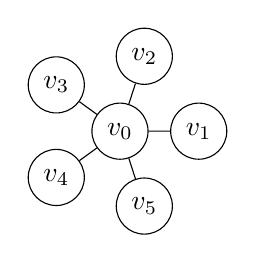
\begin{tikzpicture}
\tikzstyle{every node}=[draw,shape=circle];
\node (v0) at (0:0) {$v_0$};
\node (v1) at ( 0:1) {$v_1$};
\node (v2) at ( 72:1) {$v_2$};
\node (v3) at (2*72:1) {$v_3$};
\node (v4) at (3*72:1) {$v_4$};
\node (v5) at (4*72:1) {$v_5$};
\draw (v0) -- (v1)
(v0) -- (v2)
(v0) -- (v3)
(v0) -- (v4)
(v0) -- (v5);
\end{tikzpicture} &
\begin{lstlisting} [language={[LaTeX]TeX},basicstyle=\ttfamily]
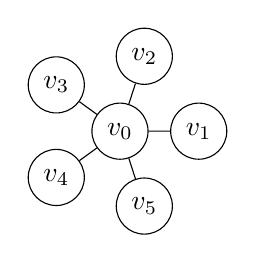
\begin{tikzpicture}
\tikzstyle{every node}=[draw,shape=circle];
\node (v0) at (0:0) {$v_0$};
\node (v1) at ( 0:1) {$v_1$};
\node (v2) at ( 72:1) {$v_2$};
\node (v3) at (2*72:1) {$v_3$};
\node (v4) at (3*72:1) {$v_4$};
\node (v5) at (4*72:1) {$v_5$};
\draw (v0) -- (v1)
(v0) -- (v2)
(v0) -- (v3)
(v0) -- (v4)
(v0) -- (v5);
\end{tikzpicture}
\end{lstlisting}\\
\hline
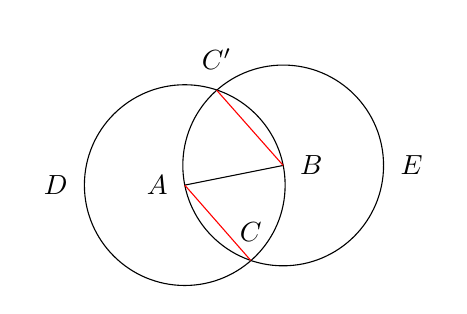
\begin{tikzpicture}
\coordinate [label=left:$A$] (A) at (0,0);
\coordinate [label=right:$B$] (B) at (1.25,0.25);
\draw (A) -- (B);
\node (D) [draw,circle through=(B),label=left:$D$] at (A) {};
\node (E) [draw,circle through=(A),label=right:$E$] at (B) {};
\coordinate[label=above:$C$] (C) at (intersection 1 of D and E);
\coordinate[label=above:$C'$] (Cp) at (intersection 2 of D and E);
\draw [red] (A) -- (C);
\draw [red] (B) -- (Cp);
\end{tikzpicture} &
\begin{lstlisting} [language={[LaTeX]TeX},basicstyle=\ttfamily]
\usetikzlibrary{calc,through}
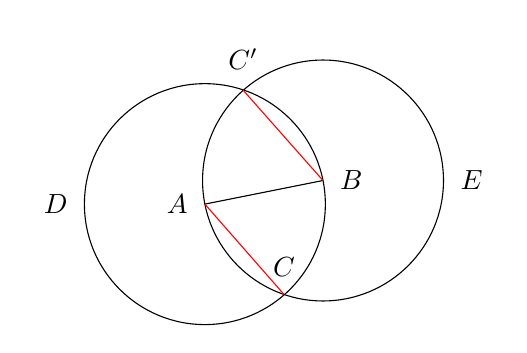
\begin{tikzpicture}[scale=1.2]
\coordinate [label=left:$A$] (A) at (0,0);
\coordinate [label=right:$B$] (B) 
 at (1.25,0.25);
\draw (A) -- (B);
\node (D) 
 [draw,circle through=(B),label=left:$D$]
 at (A) {};
\node (E) 
 [draw,circle through=(A),label=right:$E$]
 at (B) {};
\coordinate[label=above:$C$] (C) 
 at (intersection 1 of D and E);
\coordinate[label=above:$C'$] (Cp) 
 at (intersection 2 of D and E);
\draw [red] (A) -- (C);
\draw [red] (B) -- (Cp);
\end{tikzpicture}
\end{lstlisting}
\end{tabular}
\end{itemize}
\end{note}
	
\begin{note}[Loops]:\\
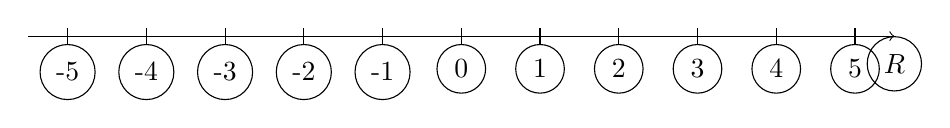
\begin{tikzpicture}
\draw[->] (-5.5,0) -- (5.5,0) node [below] {$\mathbb{R}$};
\foreach \x in {-5,...,5}
\draw (\x, 0.1) -- (\x, -0.1) node [below] {\x};
\end{tikzpicture}
\begin{lstlisting} [language={[LaTeX]TeX},basicstyle=\ttfamily]
\draw[->] (-5.5,0) -- (5.5,0) node [below] {$\mathbb{R}$};
\foreach \x in {-5,...,5}
\draw (\x, 0.1) -- (\x, -0.1) node [below] {\x};
\end{lstlisting}


\begin{tikzpicture}
\foreach \x in {1,3,...,10}
{
\shade[ball color=green!\x 0!red] (\x,0) circle (3mm);
}
\end{tikzpicture}
\begin{lstlisting} [language={[LaTeX]TeX},basicstyle=\ttfamily]
\foreach \x in {1,3,...,10}
{
\shade[ball color=green!\x 0!red] (\x,0) circle (3mm);
}
\end{lstlisting}
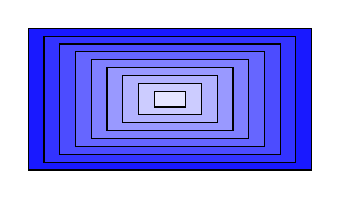
\begin{tikzpicture}
\foreach \x in {9,...,1}
\draw[fill=blue!\x0] (-0.2*\x , -0.1*\x )
rectangle (0.2*\x , 0.1*\x );
\end{tikzpicture}
\begin{lstlisting} [language={[LaTeX]TeX},basicstyle=\ttfamily]
\foreach \x in {9,...,1}
\draw[fill=blue!\x0] (-0.2*\x , -0.1*\x ) rectangle (0.2*\x , 0.1*\x );
\end{lstlisting}
\end{note}

\begin{note}[Some Samples]:\\
\begin{center}
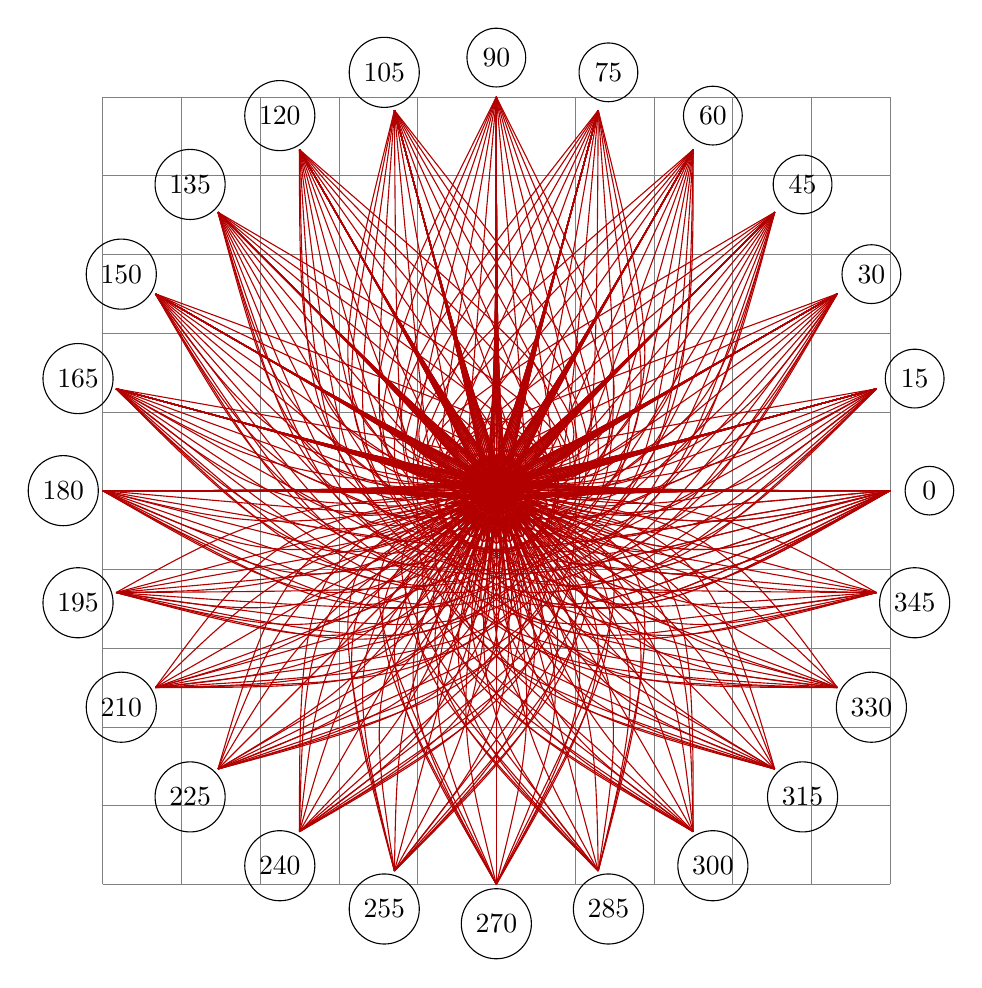
\begin{tikzpicture}
\draw[help lines] (-5,-5) grid (5,5);
\foreach \x in {0,15,...,350}
\node (n \x) at ( \x : 5.5) {\x};
\foreach \x in {0,15,...,180} 
\foreach \y in {0,15,...,360}
\draw[red!70!black] (\x:5) .. controls (\x:-2.5) .. (\y:5);
\end{tikzpicture}
\end{center}
\begin{lstlisting} [language={[LaTeX]TeX},basicstyle=\ttfamily]
\draw[help lines] (-5,-5) grid (5,5);
\foreach \x in {0,15,...,350}
\node (n \x) at ( \x : 5.5) {\x};
\foreach \x in {0,15,...,180} 
\foreach \y in {0,15,...,360}
\draw[red!70!black] (\x:5) .. controls (\x:-2.5) .. (\y:5);
\end{lstlisting}

\begin{center}

\begin{tikzpicture}[even odd rule]
\fill[clip] (0,0) circle (2cm) (60:2.5cm) arc (60:-60:2.5) (60:3cm) arc (60:-60:3cm);
\end{tikzpicture}

\begin{lstlisting} [language={[LaTeX]TeX},basicstyle=\ttfamily]

\begin{tikzpicture}[even odd rule]
\fill[clip] (0,0) circle (2cm) (60:2.5cm) 
arc (60:-60:2.5) (60:3cm) arc (60:-60:3cm);
\end{tikzpicture}
\end{lstlisting}
\end{center}

\begin{center}
	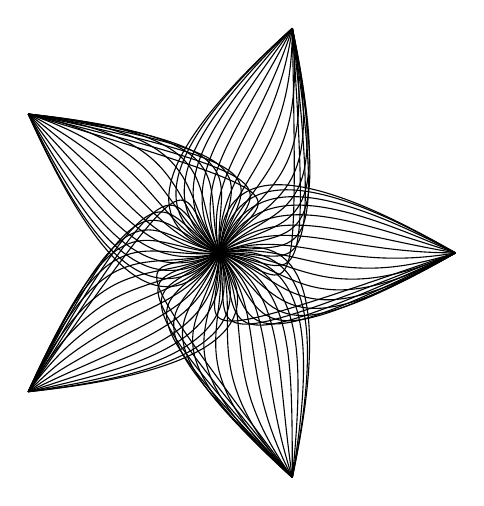
\begin{tikzpicture}
	\foreach \y in {0,360/5,2*360/5,3*360/5,4*360/5}
	\foreach \x in {-90,-80,...,90}
	\draw (0,0) .. controls (\x+\y:1) and (\x+\y-30:1.5) .. (\y:3);
	\end{tikzpicture}
	
	\begin{lstlisting} [language={[LaTeX]TeX},basicstyle=\ttfamily]
\foreach \y in {0,360/5,2*360/5,3*360/5,4*360/5}
\foreach \x in {-90,-80,...,90}
\draw (0,0) .. controls (\x+\y:1) and (\x+\y-30:1.5) .. (\y:3);
	\end{lstlisting}
\end{center}
\begin{center}
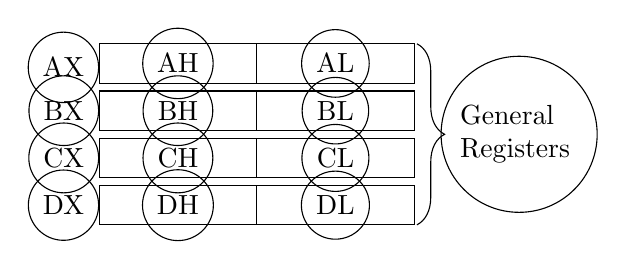
\begin{tikzpicture}
\node[left] at (0,0.25) {DX};
\draw (0,0) rectangle (2,.5) node [pos=0.5] {DH};
\draw (2,0) rectangle (4,.5) node [pos=0.5] {DL};

\node[left] at (0,0.85) {CX};
\draw (0,0.6) rectangle (2,1.1) node [pos=0.5] {CH};
\draw (2,0.6) rectangle (4,1.1) node [pos=0.5] {CL};

\node[left] at (0,1.45) {BX};
\draw (0,1.2) rectangle (2,1.7) node [pos=0.5] {BH};
\draw (2,1.2) rectangle (4,1.7) node [pos=0.5] {BL};

\node[left] at (0,2) {AX};
\draw (0,1.8) rectangle (2,2.3) node [pos=0.5] {AH};
\draw (2,1.8) rectangle (4,2.3) node [pos=0.5] {AL};

\draw [decorate,decoration={brace,amplitude=10pt,mirror},xshift=1pt,yshift=0pt]
(4,0) -- (4,2.3) node [black,midway,right,xshift=0.3cm,text width=1.5cm] 
{General Registers};
\end{tikzpicture}
\begin{lstlisting}[language={[LaTeX]TeX},basicstyle=\ttfamily]
\node[left] at (0,0.25) {DX};
\draw (0,0) rectangle (2,.5) node [pos=0.5] {DH};
\draw (2,0) rectangle (4,.5) node [pos=0.5] {DL};

\node[left] at (0,0.85) {CX};
\draw (0,0.6) rectangle (2,1.1) node [pos=0.5] {CH};
\draw (2,0.6) rectangle (4,1.1) node [pos=0.5] {CL};

\node[left] at (0,1.45) {BX};
\draw (0,1.2) rectangle (2,1.7) node [pos=0.5] {BH};
\draw (2,1.2) rectangle (4,1.7) node [pos=0.5] {BL};

\node[left] at (0,2) {AX};
\draw (0,1.8) rectangle (2,2.3) node [pos=0.5] {AH};
\draw (2,1.8) rectangle (4,2.3) node [pos=0.5] {AL};

\draw [decorate,decoration={brace,amplitude=10pt,mirror}
 ,xshift=1pt,yshift=0pt]
(4,0) -- (4,2.3) node [black,midway,right,xshift=0.3cm,text width=1.5cm] 
{General Registers};
\end{lstlisting}
\end{center}
\end{note}

